\newpage
\section{ADC}
    \subsection{Erklärung}
    Der STM hat einen ADC eingebaut, dieser kann bei den größeren Packages sogar als Temperatursensor verwendet werden.
    Alle GPIOs können als ADC Eingang verwendet werden solange sie als analog GPIO konfiguriert werden. 
    
    \subsection{Register}
        Die Register für den ADC beginnen bei 0x4001 2400 bis 0x4001 27FF.
        Für die Konfiguration werden folgende Register benötigt:

        \subsubsection{ADC\_ISR | ADC Interrupts}
            \begin{figure}[!htb]
                \centering
                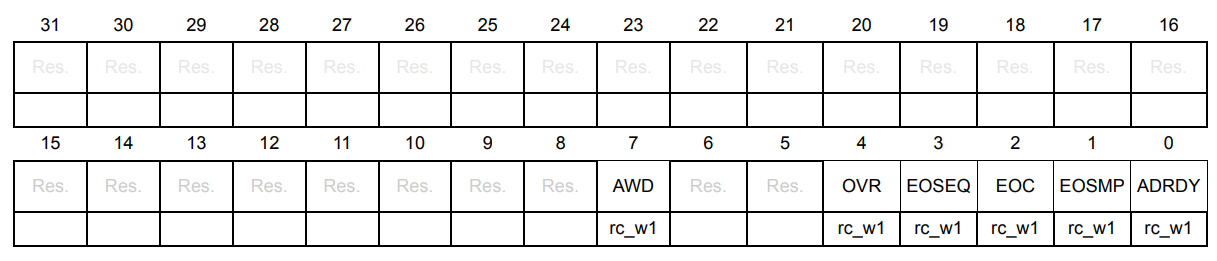
\includegraphics[width=\linewidth]{ADC-ISR-Register.png}
                \caption{ADC-ISR-Register}
                \label{caption:ADC-ISR-Register}
            \end{figure}
             
            \begin{itemize}
                \item EOC (End of conversion):\\
                0: Channel conversion not complete (or the flag event was already acknowledged and cleared by
                software)\\
                1: Channel conversion complete
                \item ADRDY (ADC ready):
                0: ADC not yet ready to start conversion (or the flag event was already acknowledged and cleared
                by software)\\
                1: ADC is ready to start conversion
            \end{itemize}
            
\newpage
        \subsubsection{ADC\_IER | ADC enable Interrupts}
            \begin{figure}[!htb]
                \centering
                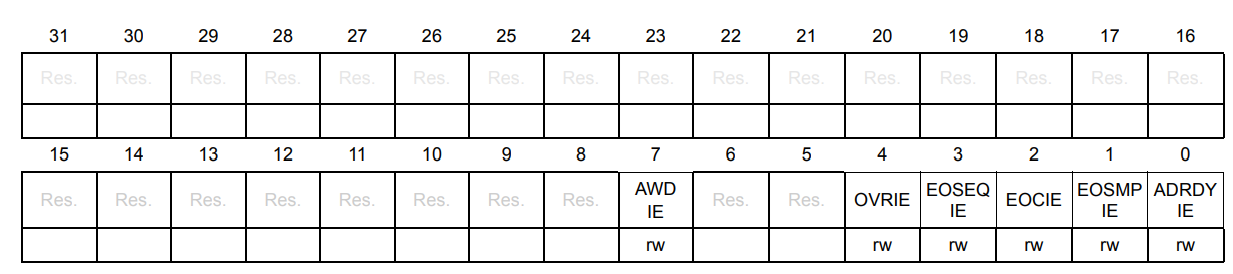
\includegraphics[width=\linewidth]{ADC-IER-Register.png}
                \caption{ADC-IER-Register}
                \label{caption:ADC-IER-Register}
            \end{figure}
            \noindent Benötigt wird:
            \begin{itemize}
                \item EOCIE(End of conversion interrupt enable):\\
                0: EOC interrupt disabled\\
                1: EOC interrupt enabled. An interrupt is generated when the EOC bit is set.
                \item ADRDYIE (ADC ready interrupt enable):
                0: ADRDY interrupt disabled.\\
                1: ADRDY interrupt enabled. An interrupt is generated when the ADRDY bit is set.
            \end{itemize}



        \subsubsection{ADC\_CR | ADC kalibrieren, aktivieren, starten}
            \begin{figure}[!htb]
                \centering
                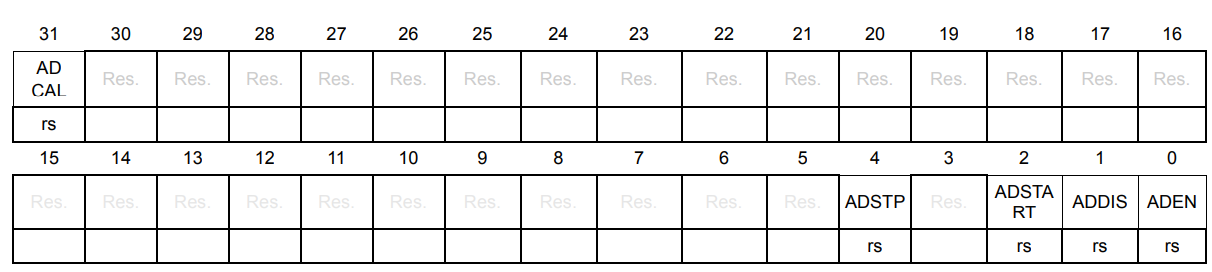
\includegraphics[width=\linewidth]{ADC-CR-Register.png}
                \caption{ADC-CR-Register}
                \label{caption:ADC-CR-Register}
            \end{figure}
            \noindent Benötigt wird:
            \begin{itemize}
                \item ADCAL (ADC calibration):\\
                0: Calibration complete \\
                1: Write 1 to calibrate the ADC. Read at 1 means that a calibration is in progress.
                \item ADEN (ADC enable command)\\
                0: ADC is disabled (OFF state)\\
                1: Write 1 to enable the ADC. 
                \item ADSTART (ADC start conversion command)\\
                0: No ADC conversion is ongoing. \\
                1: Write 1 to start the ADC. Read 1 means that the ADC is operating and may be converting
            \end{itemize}

\newpage
        \subsubsection{ADC\_CFGR2 | Clock Einstellung}
            \begin{figure}[!htb]
                \centering
                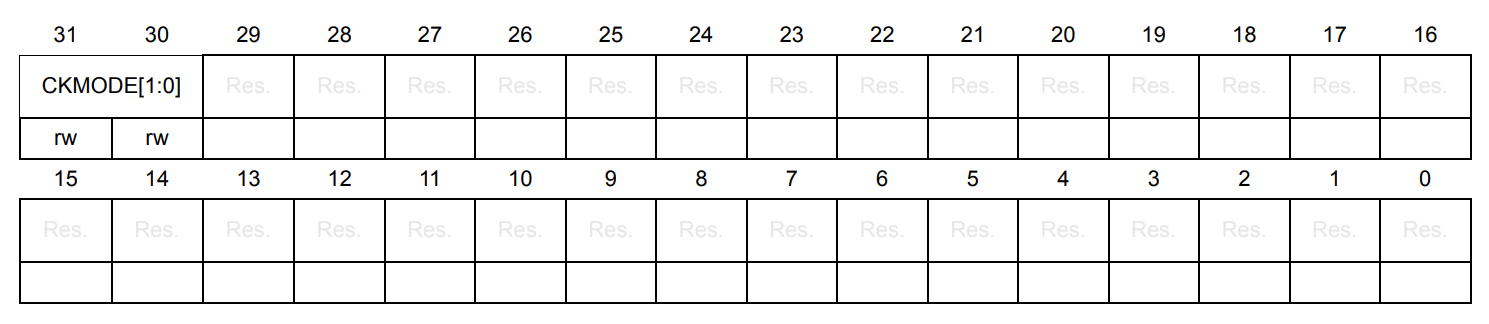
\includegraphics[width=\linewidth]{ADC-CFGR2-Register.png}
                \caption{ADC-CFGR2-Register}
                \label{caption:ADC-CFGR2-Register}
            \end{figure}
            \noindent Benötigt wird:
            \begin{itemize}
                \item CKMODE[1:0] (ADC clock mode):\\
                00: ADCCLK (Asynchronous clock mode), generated at product level (refer to RCC section)\\
                01: PCLK/2 (Synchronous clock mode)\\
                10: PCLK/4 (Synchronous clock mode)\\
                11: Reserved
            \end{itemize}


        \subsubsection{ADC\_CHSELR | ADC Input Channel}
            \begin{figure}[!htb]
                \centering
                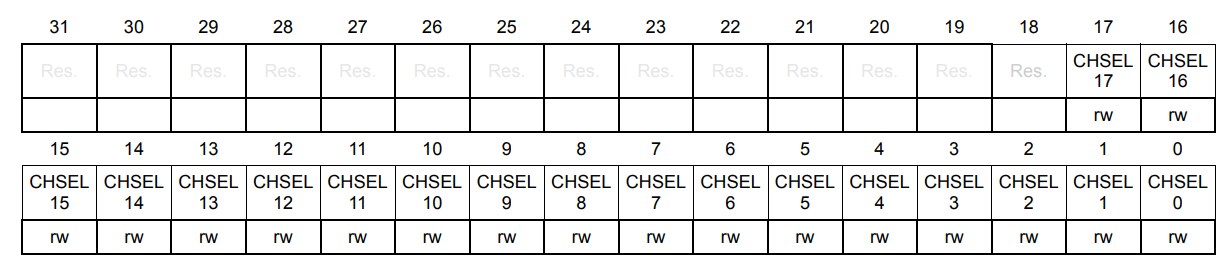
\includegraphics[width=\linewidth]{ADC-CHSELR-Register.png}
                \caption{ADC-CHSELR-Register}
                \label{caption:ADC-CHSELR-Register}
            \end{figure} 
            \noindent Benötigt wird:
            \begin{itemize}
                \item CHSELx: Channel-x selection\\
                0: Input Channel-x is not selected for conversion\\
                1: Input Channel-x is selected for conversion
            \end{itemize}

\newpage
        \subsubsection{ADC\_DR | 16 Bit Ergebniss der Umnwandlung}
            \begin{figure}[!htb]
                \centering
                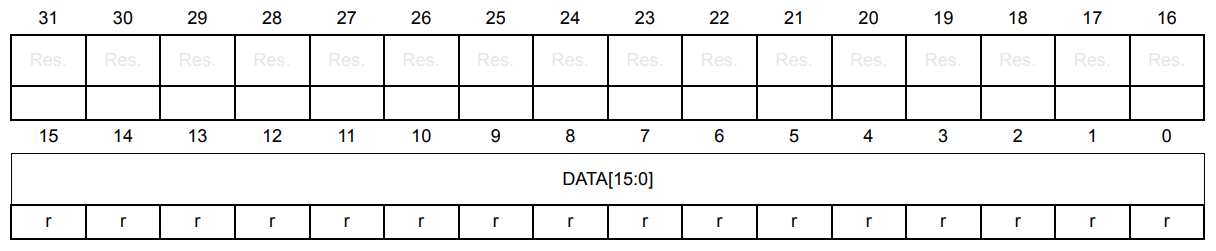
\includegraphics[width=\linewidth]{ADC-DR-Register.png}
                \caption{ADC-DR-Register}
                \label{caption:ADC-DR-Register}
            \end{figure}
            \noindent Benötigt wird:
            \begin{itemize}
                \item DATA[15:0]: Converted data
            \end{itemize}
            
        
        
    
    \subsection{Konfiguration}
        Um den ADC zu konfigurieren, wird zuerst der ADC Clock eingestellt $\rightarrow$ der ADC kalibriert $\rightarrow$  
        ADC aktiviert $\rightarrow$  GPIO als ADC Input einstellen.\\
        Wenn die Kalibrierung fertig ist, ist das ADCAL Bit 0. Dann kann der ADC und Interrupts aktiviert werden und eingestellt werden 
        welcher GPIO Pin als Input verwendet wird. Weiterhin wird der ADC im vortlaufenden (continuous) Modus betrieben, sodass im EOC Interrupt die Umwandlung nicht 
        wieder gestartet werden muss. \\\\
        
        \noindent Danach wenn der ADC bereit ist wird im Interrupt Register die ADC\_ADRDY (ADC Ready) flag gesetzt, dieses wird im ADC-Interrupt-Handler abgefragt und dann
        eine Umwandlung gestartet.\\ 
        Wenn eine Umwandlung fertig ist wird im Interrupt Register das ADC\_TC (Transmission complete) flag gesetzt. Im ADC-Interrupt-Hanlder wird dann aus dem ADC\_DR Register
        das Ergebniss der Umwandlung weitergeben um dies dann an der USART senden zu können.
    
\newpage
    \subsection{ADC-Initiallisierungs-Code}
        \begin{lstlisting}[language=C, style=CStyle, caption=ADC-Initiallisierungs-Code, captionpos=b, label=ADC-Initiallisierungs-Code]
int init_ADC()
{   
    uint32_t reg_content;
    uint32_t* adc_chselr = ADC_CHSELR;
    uint32_t* adc_isr = ADC_ISR;       
    uint32_t* adc_cr = ADC_CR;
    uint32_t* adc_cfgr1 = ADC_CFGR1;
    uint32_t adc_cr_adcal = ADC_CR_ADCAL;
    uint32_t* adc_ier = ADC_IER;
    uint32_t* adc_cfgr2 = ADC_CFGR2;
    uint32_t adc_isr_adrdy = ADC_ISR_ADRDY;
    
    //set ADC clock to PCLK so thats is synchronous with sysclock
    reg_content = *adc_cfgr2;
    reg_content |= 0x40000000;
    *adc_cfgr2 = reg_content;
    //before starting callibrate ADC
    reg_content = *adc_cr;
    reg_content |= adc_cr_adcal;
    *adc_cr = reg_content;

    //if calibration is complete enable ADC
    //enable Interrupts
    //set correct channel
    //when ADC is ready, a ad ready interrupt occurs and the interrupt handler
    //will then start the ADC convertion
    while((*adc_cr & adc_cr_adcal) == adc_cr_adcal); // wait till callibration is complete

    //enable ADC and ensure ADSTART=0 for further configuration and enable ADC
    reg_content = *adc_cr;
    reg_content |= 0x00000001;
    *adc_cr = reg_content;
    //set ADC to continues convertion so, that convertion doesn't to start again in Interrupt
    reg_content = *adc_cr;
    reg_content |= 0x0000200;
    *adc_cr = reg_content;
    //enable Interrupts of ADC
    reg_content = *adc_ier;
    reg_content |= 0x00000005;
    *adc_ier = reg_content;
    //Set ADC Channel to channel 0 because PA0 is ADC_IN0
    reg_content = *adc_chselr;
    reg_content |= 0x00000001;
    *adc_chselr = reg_content;
}
        \end{lstlisting}
\newpage
    \subsection{ADC-Interrupt-Handler-Code}
        \begin{lstlisting}[language=C, style=CStyle, caption=ADC-Interrupt-Handler-Code, captionpos=b, label=ADC-Interrupt-Handler-Code]
void ADC1_IRQHandler(void)   
{
    uint32_t* adc_isr = ADC_ISR;
    uint32_t* adc_cr = ADC_CR;

    uint32_t adc_isr_eoc = ADC_ISR_EOC;
    uint32_t adc_isr_adrdy = ADC_ISR_ADRDY;
    uint32_t* adc_dr = ADC_DR;
    uint32_t adc_dr_data = ADC_DR_DATA;
    uint32_t* gpioa_odr = GPIOA_ODR;
    uint32_t* usart1_tdr =  USART1_TDR;
    
    uint32_t adc_cr_adstart = ADC_CR_ADSTART;
    uint16_t ADC_Value;
    
    uint32_t reg_content;

    //if ADC Ready start convertion
    if((*adc_isr & adc_isr_adrdy) == adc_isr_adrdy)
    {
        reg_content = *adc_cr;
        reg_content |= adc_cr_adstart;
        *adc_cr = reg_content;
    }

    //if convertion complete send ADC value
    if((*adc_isr & adc_isr_eoc) == adc_isr_eoc)
    {
        send=0;
        ADC_Value = (*adc_dr & adc_dr_data);
        //Set PA7 and PA6 high for max to send data
        reg_content = *gpioa_odr;
        reg_content |= 0x000000C0;
        *gpioa_odr = reg_content;
        
        sprintf(USART_write_data, "%d", ADC_Value);
    
        //write something into the USART Buffer for USART
        //interrupt where rest of adc value gets put into the buffer
        *usart1_tdr = 'n'; 
    }
}
        \end{lstlisting}